% =====================================================================
%  Shared sections (model, stability, control, swing-up) used by build_full_report.py and build_phase_reports.py
%  (layout follows the senior reference report: title page, contents,
%   numbered sections, code listings, tabulation, conclusion, contributions)
% =====================================================================
\documentclass[12pt,a4paper]{article}
\usepackage[a4paper,margin=1in]{geometry}
\usepackage[T1]{fontenc}
\usepackage{lmodern}
\usepackage{amsmath,amssymb,bm}
\usepackage{graphicx,float,booktabs,array,multirow}
\usepackage{xcolor}
\usepackage{algorithm}
\usepackage{algpseudocode}
\usepackage{fancyhdr}
\usepackage{enumitem}
\usepackage{caption}
\usepackage[hidelinks]{hyperref}

\pagestyle{fancy}
\fancyhf{}
\renewcommand{\headrulewidth}{0.6pt}
\fancyfoot[C]{\thepage}
\setlength{\headheight}{14.5pt}
\setlength{\parskip}{4pt}
\setlength{\parindent}{0pt}
\newcommand{\Nm}{\,\mathrm{N\,m}}
\captionsetup{font=small}

\begin{document}

\begin{titlepage}
\centering
\vspace*{2cm}

\includegraphics[width=4.2cm]{figures/logo-000.jpg}\\[3cm]
{\Huge Systems Thinking Project}\\[0.5cm]
{\Large Acrobot}\\[0.25cm]
{\large Phase 4: Swing-Up}\\[2.2cm]
\begin{tabular}{cc}
\textbf{Author:} Bhargav & \textbf{Author:} Sreekar\\
ID: 2025102061 & ID: 2025102074\\[0.8cm]
\textbf{Author:} Kaushik & \textbf{Author:} Divijat\\
ID: 2025102071 & ID: 2025102040
\end{tabular}
\vfill
{\large November 11, 2026}
\end{titlepage}

\tableofcontents
\newpage

\section{Introduction}
% =====================================================================
\subsection{What is an Acrobot?}
An acrobot is a two-link pendulum that hangs from a fixed pivot. The first link (the ``shoulder'' link) is free to rotate about the pivot; the second link is joined to the end of the first at the ``elbow''. The only motor sits at the elbow, so the shoulder is \emph{passive}. It is the robot version of a gymnast on a high bar who can only swing the legs at the hips. Because there are two degrees of freedom but only one actuator, the acrobot is a standard example of an \emph{underactuated} system [1], [2].

\subsection{Model}
The configuration is described by two generalised coordinates: $q_1$, the angle of link~1 from the downward vertical, and $q_2$, the angle of link~2 relative to link~1. The full state contains the angles and their rates:
\[
\mathbf q=\begin{bmatrix}q_1\\q_2\end{bmatrix},\qquad
\mathbf x=\begin{bmatrix}q_1\\q_2\\\dot q_1\\\dot q_2\end{bmatrix}.
\]
\begin{figure}[H]
\centering
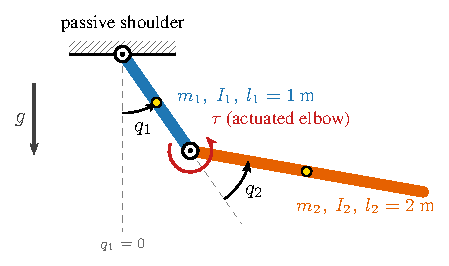
\includegraphics[width=0.42\textwidth]{figures/acrobot_diagram.pdf}
\caption{The acrobot: passive shoulder at the pivot, motor torque $\tau$ at the elbow; dots mark the centres of mass.}
\label{fig:acrobot}
\end{figure}

\subsection{Equations of Motion}
The dynamics (given in the Phase~1 helper and verified in Phase~1) are
\begin{equation}
M(q)\,\ddot q+C(q,\dot q)\,\dot q=\tau_g(q)+B\,\tau,\qquad B=\begin{bmatrix}0\\1\end{bmatrix},\qquad |\tau|\le 20\Nm .\label{eq:eom}
\end{equation}

\textbf{$\tau$ (Input Torque):} the torque of the elbow motor, the only quantity we command. $B=[0,\,1]^T$ says it acts on the elbow equation only.

\textbf{$M(q)$ (Inertia Matrix):} the resistance to angular acceleration. It depends on the elbow angle because the mass distribution changes as the arm folds:
\begin{equation}
M(q)=\begin{bmatrix}2.663+2\cos q_2 & 1.33+\cos q_2\\ 1.33+\cos q_2 & 1.33\end{bmatrix},\qquad \det M=1.7729-\cos^2q_2\ge0.7729>0 .
\end{equation}

\textbf{$C(q,\dot q)$ (Coriolis Matrix):} the coupling forces between the links (centrifugal and Coriolis effects):
\begin{equation}
C(q,\dot q)=\sin q_2\begin{bmatrix}-2\dot q_2 & -\dot q_2\\ \dot q_1 & 0\end{bmatrix}.
\end{equation}

\textbf{$\tau_g(q)$ (Gravity Torque):} the torque that gravity exerts on each joint, $\tau_g=-\partial U/\partial q$, with potential energy $U$:
\begin{equation}
U=-14.715\cos q_1-9.81\cos(q_1+q_2),\qquad
\tau_g(q)=-9.81\begin{bmatrix}1.5\sin q_1+\sin(q_1+q_2)\\ \sin(q_1+q_2)\end{bmatrix}.
\end{equation}

\textbf{System Parameters:}
\begin{gather*}
m_1=m_2=1\,\mathrm{kg},\qquad l_1=1\,\mathrm m,\qquad l_2=2\,\mathrm m,\qquad l_{c1}=0.5\,\mathrm m,\qquad l_{c2}=1\,\mathrm m,\\
I_1=0.083\,\mathrm{kg\,m^2},\qquad I_2=0.33\,\mathrm{kg\,m^2},\qquad g=9.81\,\mathrm{m\,s^{-2}}.
\end{gather*}

\subsection{Equilibria and Linear Model (from Phase 1)}
With $\tau^*=0$ the equilibria satisfy $\tau_g(q^*)=0$, i.e.\ $\sin q_1^*=0$ and $\sin(q_1^*+q_2^*)=0$. This gives four postures:
\begin{table}[H]
\centering
\caption{The four equilibria}
\begin{tabular}{|c|c|c|c|l|}
\hline
 & Posture & $(q_1^*,q_2^*)$ & $U$ [J] & Description\\ \hline
$E_1$ & down--down & $(0,0)$ & $-24.525$ & both links hanging\\
$E_2$ & down--up & $(0,\pi)$ & $-4.905$ & link 1 down, link 2 up\\
$E_3$ & up--up & $(\pi,0)$ & $+24.525$ & fully upright (target)\\
$E_4$ & up--down & $(\pi,\pi)$ & $+4.905$ & link 1 up, link 2 down\\ \hline
\end{tabular}
\end{table}
Linearizing about each equilibrium with $\tilde x=x-x^*$ gives
\begin{equation}
\dot{\tilde x}=A\tilde x+B_\ell\tilde\tau,\qquad A=\begin{bmatrix}0&I\\P&0\end{bmatrix},\qquad B_\ell=\begin{bmatrix}0\\r\end{bmatrix},\label{eq:lin}
\end{equation}
with $P=M(q^*)^{-1}K(q^*)$ and $r=M(q^*)^{-1}B$,
where $K=\partial\tau_g/\partial q$. The transfer functions from $\tau$ to the angles are
\begin{gather}
G_1(s)=\frac{r_1s^2+(P_{12}r_2-P_{22}r_1)}{\Delta(s)},\qquad
G_2(s)=\frac{r_2s^2+(P_{21}r_1-P_{11}r_2)}{\Delta(s)},\label{eq:tf}\\
\Delta(s)=s^4-\operatorname{tr}(P)\,s^2+\det P .\nonumber
\end{gather}
\begin{table}[H]
\centering
\caption{Transfer functions at the four equilibria (Phase 1)}
\label{tab:tf}
\small
\begin{tabular}{|c|l|l|l|}
\hline
 & $\Delta(s)$ & $N_1(s)$ ($\tau\to q_1$) & $N_2(s)$ ($\tau\to q_2$)\\ \hline
$E_1$ & $s^4+42.2410\,s^2+186.7719$ & $-3.0147\,(s^2+4.2103)$ & $6.0332\,(s^2+5.2595)$\\
$E_2$ & $s^4+8.4025\,s^2-186.7719$ & $-0.4270\,(s^2-29.7273)$ & $0.8578\,(s^2+7.3982)$\\
$E_3$ & $s^4-42.2410\,s^2+186.7719$ & $-3.0147\,(s^2-4.2103)$ & $6.0332\,(s^2-5.2595)$\\
$E_4$ & $s^4-8.4025\,s^2-186.7719$ & $-0.4270\,(s^2+29.7273)$ & $0.8578\,(s^2-7.3982)$\\ \hline
\end{tabular}
\end{table}

\subsection{Objective}
Starting from hanging straight down ($E_1$), bring the acrobot to the upright equilibrium $E_3$ and hold it, with $|\tau|\le20\Nm$. Whether the attempt works or not, explain with evidence why it behaved as it did.

Phase~3 provides the controller that holds the upright: LQR with $Q=I$, $R=0.03$, $K=[-503.0,\,-203.9,\,-218.3,\,-101.5]$. It recovers only from a thin region around $E_3$ ($6^\circ$ in $q_1$, $13^\circ$ in $q_2$), so the swing-up must deliver the arm into that region.

% =====================================================================
\section{Swing-Up}
% =====================================================================
\subsection{Energy Target}
Hanging has $E=U(E_1)=-24.525$~J and the upright needs $E_{top}=U(E_3)=+24.525$~J. The controller must therefore add $49$~J with a $20\Nm$ elbow motor, and deliver the arm close enough to $E_3$ for the Phase~3 LQR to catch it.

\subsection{Swing-Up Controller}
\textbf{Partial feedback linearization.} With $h=C\dot q-\tau_g$, row~1 of~\eqref{eq:eom} gives $\ddot q_1=-(M_{12}\ddot q_2+h_1)/M_{11}$. Substituting into row~2, the elbow follows any desired acceleration $v$ exactly:
\begin{equation}
\tau=\Big(M_{22}-\frac{M_{21}M_{12}}{M_{11}}\Big)v+h_2-\frac{M_{21}h_1}{M_{11}}\ \Rightarrow\ \ddot q_2=v .
\end{equation}
\textbf{Energy pumping.} The desired elbow acceleration is
\begin{equation}
v=-k_1\tilde q_2-k_2\dot q_2+k_3\,\dot q_1\,(E-E_{top}) .\label{eq:v}
\end{equation}
\begin{itemize}
\item $k_1$, $k_2$: keep the elbow nearly straight (a stiff and damped elbow).
\item $k_3$: pushes in step with $\dot q_1$ while $E<E_{top}$ (adds energy) and against it when $E>E_{top}$ (removes energy), like a child pumping a swing.
\end{itemize}

\subsection{Hybrid Switching}
\begin{equation}
\tau=\operatorname{sat}\begin{cases}-K\tilde x, & \tilde x^TS\tilde x<c_{sw}=5\quad\text{(catch: Phase 3 LQR at $E_3$)}\\ \text{swing-up law above}, & \text{otherwise}\end{cases}
\end{equation}
If the arm leaves the catch region (a missed catch or a push), swing-up resumes automatically.

\subsection{Choice of Gains}
We searched 144 designs ($k_1\in\{20,50,100\}$, $k_2\in\{2,5,10\}$, $k_3\in\{0.3,1,3,10\}$, $c_{sw}\in\{0.5,1,2,5\}$) from $0.05$~rad off hanging; 22 swung up and held. Each was then rerun from 40 random starts. \textbf{$k=(20,2,3)$, $c_{sw}=5$} succeeded from \textbf{39/40}, with a median first catch of $4.0$~s.

\subsection{Results}
\begin{table}[H]
\centering
\caption{Swing-up runs in PyBullet ($|\tau|\le20\Nm$)}
\label{tab:swing}
\small
\resizebox{\textwidth}{!}{\begin{tabular}{|l|c|c|c|c|}
\hline
Start (from hanging) & First catch & Final deviation from $E_3$ & Torque saturated & Result\\ \hline
$(3^\circ,0)$, $k=(20,2,3)$ & $2.2$ s & $<0.001^\circ$ & 5\% & held\\
$(-10^\circ,20^\circ)$, $k=(20,2,3)$ & $9.5$ s & $<0.01^\circ$ & 17\% & held\\
$(3^\circ,0)$, kick $0.8$ rad/s at 8 s & $2.2$ s, re-caught & $<0.001^\circ$ & 5\% & held\\
$(3^\circ,0)$, textbook $k=(50,5,10)$ & $8.4$ s & $<0.001^\circ$ & 7\% & held (this start)\\ \hline
\end{tabular}}
\end{table}
\begin{figure}[H]
\centering
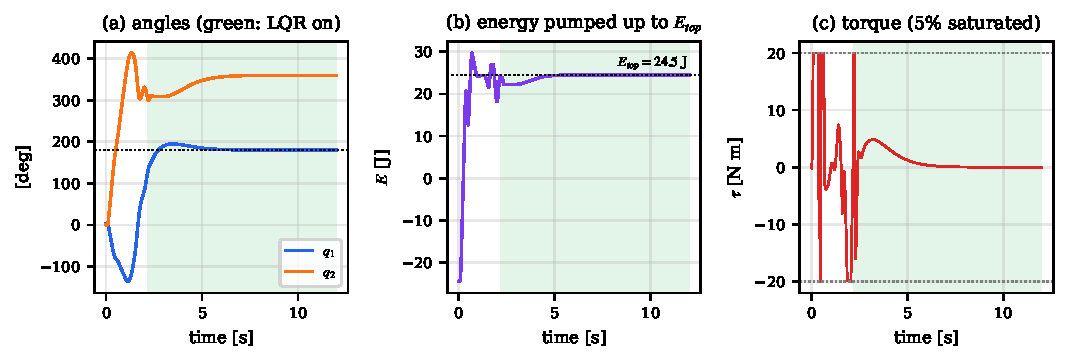
\includegraphics[width=\textwidth]{figures/fig_swingup.pdf}
\caption{Swing-up from $3^\circ$: (a) angles, (b) energy pumped to $E_{top}$, (c) torque. Green: LQR active.}
\label{fig:swingup}
\end{figure}

\subsection{Why It Works, and Why Other Gains Fail}
\begin{table}[H]
\centering
\caption{Success from 40 random starts vs.\ saturation during swing-up}
\label{tab:sat}
\begin{tabular}{|l|c|c|}
\hline
Gains $(k_1,k_2,k_3)$, $c_{sw}$ & Swing-up time at $|\tau|=20$ & Held (of 40)\\ \hline
$(20,2,3)$, 5 (chosen) & 26\% & \textbf{39}\\
$(50,2,3)$, 5 & 38\% & 4\\
$(100,2,3)$, 5 & 45\% & 2\\
$(20,2,0.3)$, 5 & 25\% & 0\\
$(50,5,10)$, 5 (textbook) & 33\% & 25\\
$(50,5,10)$, 1 (textbook) & 31\% & 13\\ \hline
\end{tabular}
\end{table}
\begin{enumerate}
\item \textbf{Saturation breaks the swing-up law.} The law assumes the full linearizing torque is applied. A stiff elbow (large $k_1$) asks for more than $20\Nm$ more often (26\% $\to$ 45\% of the time). While saturated $\ddot q_2\ne v$, the energy is no longer steered precisely, and the arm reaches the top off the catch region. Success drops from 39 to 2.
\item \textbf{Too little pumping.} With $k_3=0.3$ the energy approaches $E_{top}$ too slowly to reach the catch region within 40~s (0/40).
\item \textbf{The catch is the Phase 3 limit.} The LQR recovers only a thin region around $E_3$. The swing-up only has to deliver the arm into that region, and $c_{sw}=5$ was the most reliable threshold tried.
\item \textbf{Retry.} Because swing-up resumes whenever $\tilde x^TS\tilde x\ge c_{sw}$, a missed catch or a push costs time, not the task (Fig.~\ref{fig:kick}a).
\end{enumerate}
\begin{figure}[H]
\centering
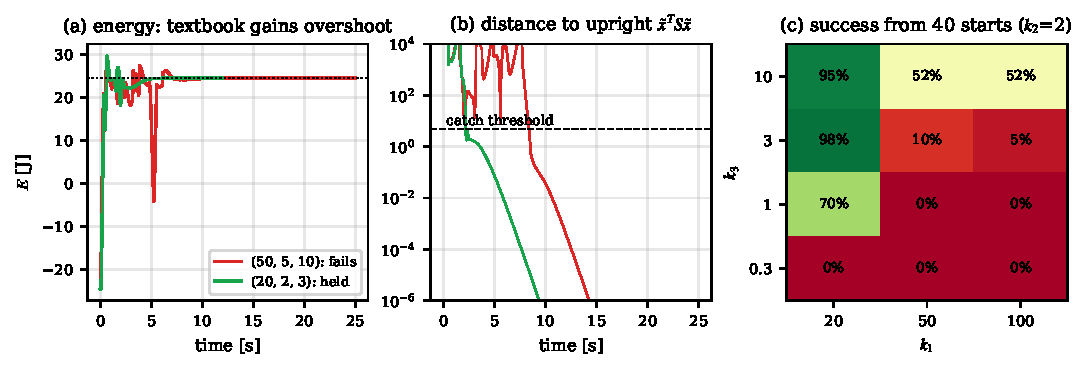
\includegraphics[width=\textwidth]{figures/fig_why.pdf}
\caption{(a) Energy, chosen vs.\ textbook gains; (b) distance to the upright and the catch threshold; (c) success rate over $(k_1,k_3)$.}
\label{fig:why}
\end{figure}
\begin{figure}[H]
\centering
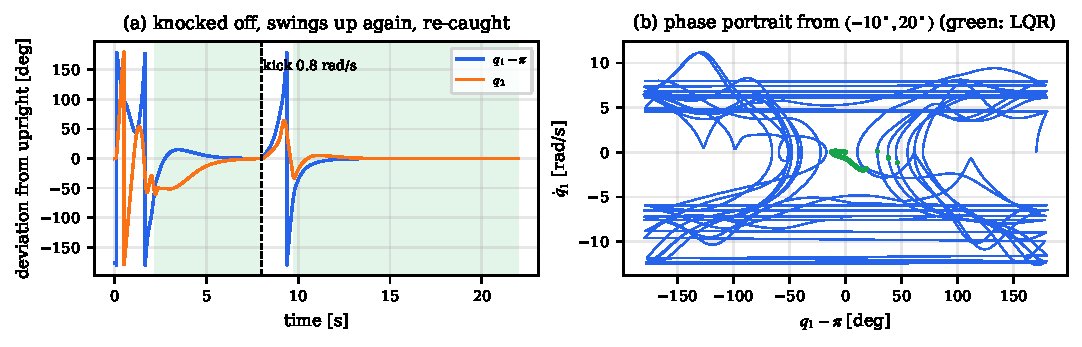
\includegraphics[width=0.9\textwidth]{figures/fig_kick.pdf}
\caption{(a) Knocked off at 8~s, swung up and caught again; (b) phase portrait from $(-10^\circ,20^\circ)$, green where LQR is active.}
\label{fig:kick}
\end{figure}

% =====================================================================
% =====================================================================
\section{Simulations and Code}
% =====================================================================
\subsection{PyBullet Simulator}
All simulations use the full nonlinear model in PyBullet with an interactive dashboard (Fig.~\ref{fig:dash}). The user picks an equilibrium, an initial condition (slider, typed value or by dragging the arm) and a controller: swing-up $\to$ LQR, or any of the Phase 2 and 3 controllers. The dashboard shows $\tilde q(t)$, $\tau(t)$ and the closed-loop poles live. File: \texttt{phase4/acrobot\_phase4\_sim.py}; instructions in \texttt{phase4/README.md}.
\begin{figure}[H]
\centering
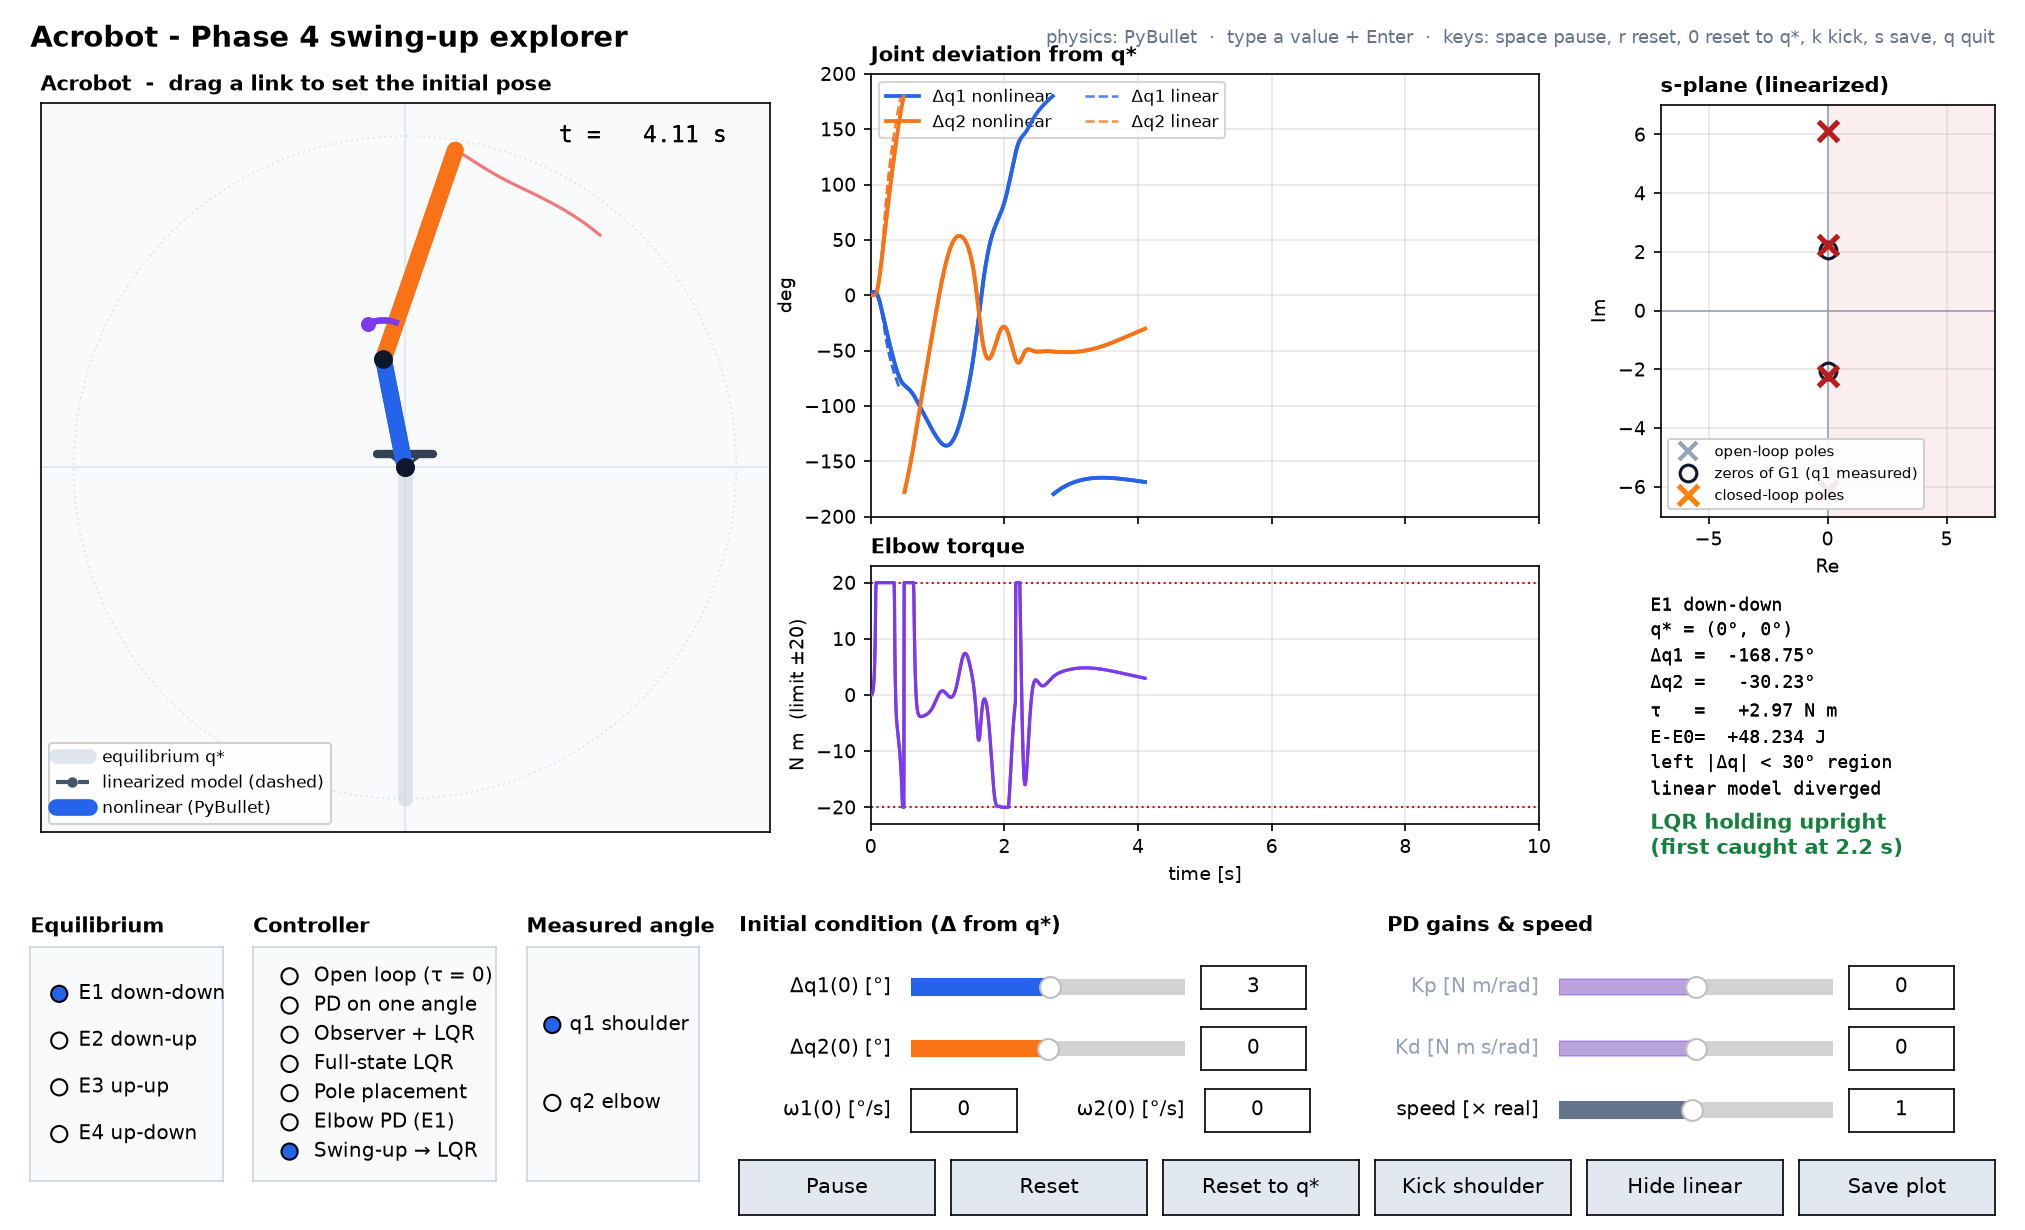
\includegraphics[width=\textwidth]{figures/dashboard.png}
\caption{Phase 4 dashboard during a swing-up from hanging.}
\label{fig:dash}
\end{figure}

\subsection{MATLAB Codes}
It runs the hybrid controller from three starts (RK4, 1~ms) and the 40-start robustness test: 39/40 for the chosen gains, as in the tables above.

The files are listed below; the algorithms they implement follow as pseudo-code.
\begin{table}[H]
\centering
\caption{MATLAB files}
\resizebox{\textwidth}{!}{\begin{tabular}{|l|l|}
\hline
File & Purpose\\ \hline
\texttt{Acrobot\_Nonlinear\_Dynamics.m} & nonlinear model $\dot x=f(x,\tau)$ with the $20\Nm$ limit (Phase 1)\\
\texttt{Acrobot\_Linearize.m} & $A$, $B_\ell$ at an equilibrium (Phase 1)\\
\texttt{Acrobot\_Phase4\_Controller.m} & hybrid swing-up $\to$ LQR controller\\
\texttt{Acrobot\_Phase4\_Main.m} & swing-up runs and the 40-start robustness test\\ \hline
\end{tabular}}
\end{table}

\begin{algorithm}[H]
\caption{Nonlinear dynamics $\dot x=f(x,\tau)$ (\texttt{Acrobot\_Nonlinear\_Dynamics.m}) and linearization (\texttt{Acrobot\_Linearize.m})}
\label{alg:model}
\begin{algorithmic}[1]
\Function{Dynamics}{$x=[q_1,q_2,\dot q_1,\dot q_2]$, $\tau$}
  \State $\tau\gets\max(-20,\min(20,\tau))$ \Comment{motor limit}
  \State build $M(q)$, $C(q,\dot q)$ and $\tau_g(q)$ from the given model
  \State solve $M\,\ddot q=\tau_g+B\tau-C\dot q$ for $\ddot q$ \Comment{backslash, never $M^{-1}$}
  \State \Return $[\dot q;\ \ddot q]$
\EndFunction
\Function{Linearize}{$q^*$}
  \State $K\gets\partial\tau_g/\partial q$ at $q^*$; \quad $P\gets M(q^*)^{-1}K$; \quad $r\gets M(q^*)^{-1}B$
  \State \Return $A=\begin{bmatrix}0&I\\P&0\end{bmatrix}$, $B_\ell=\begin{bmatrix}0\\r\end{bmatrix}$
\EndFunction
\end{algorithmic}
\end{algorithm}

\begin{algorithm}[H]
\caption{Hybrid swing-up controller (\texttt{Acrobot\_Phase4\_Controller.m}) and tests (\texttt{Acrobot\_Phase4\_Main.m})}
\label{alg:p4}
\begin{algorithmic}[1]
\Function{Controller}{$x$}
  \State $\tilde x\gets$ deviation of $x$ from the upright $E_3$ (angles wrapped to $\pm\pi$)
  \If{$\tilde x^TS\tilde x<c_{sw}=5$}
    \State $\tau\gets-K\tilde x$ \Comment{catch: upright LQR}
  \Else \Comment{swing-up: energy pumping}
    \State $E\gets\frac12\dot q^TM\dot q+U(q)$
    \State $v\gets-k_1\tilde q_2-k_2\dot q_2+k_3\,\dot q_1\,(E-E_{top})$
    \State $\tau\gets(M_{22}-M_{21}M_{12}/M_{11})\,v+h_2-M_{21}h_1/M_{11}$ \Comment{partial feedback linearization}
  \EndIf
  \State \Return $\operatorname{sat}(\tau)$ \Comment{$|\tau|\le20\Nm$}
\EndFunction
\For{each start (three chosen starts, then 40 random starts near hanging)}
  \State simulate with fixed-step RK4 (1 ms) for 30--40 s, calling \Call{Controller}{} every step
  \State record the first catch time, the share of time at $|\tau|=20$, and whether $E_3$ is held
\EndFor
\end{algorithmic}
\end{algorithm}


\subsection{Animation}
A 2K Manim animation of this phase: \href{https://drive.google.com/file/d/1jPQRn3W-bvUyvSKlHvYmX74bfPX9N16P/view?usp=sharing}{\textcolor{blue}{watch the video}}.

% =====================================================================
\section{Tabulation}
% =====================================================================
\begin{table}[H]
\centering
\caption{Summary of the swing-up designs (40 random starts near hanging)}
\resizebox{\textwidth}{!}{\begin{tabular}{|l|c|c|c|}
\hline
Gains $(k_1,k_2,k_3)$, $c_{sw}$ & Saturated during swing-up & Held & Median first catch\\ \hline
$(20,2,3)$, 5 (chosen) & 26\% & \textbf{39/40} & $4.0$ s\\
$(50,5,10)$, 5 (textbook) & 33\% & 25/40 & $5.5$ s\\
$(100,2,3)$, 5 (stiff elbow) & 45\% & 2/40 & --\\
$(20,2,0.3)$, 5 (weak pumping) & 25\% & 0/40 & --\\ \hline
\end{tabular}}
\end{table}

% =====================================================================
\section{Conclusion}
% =====================================================================
An energy-pumping swing-up based on partial feedback linearization brings the acrobot from hanging to the upright energy, and the Phase~3 LQR catches and holds it. With $|\tau|\le20\Nm$ the chosen gains $k=(20,2,3)$ succeed from 39 of 40 random starts, typically within about 4~s. Because swing-up resumes whenever the arm leaves the catch region, a missed catch or a push costs time, not the task.

The textbook gains, and stiffer elbow gains in general, do worse because they ask for more torque than the motor can give. Once the torque saturates, the elbow no longer follows the linearizing law, the energy is no longer steered precisely, and the arm reaches the top outside the small region the LQR can catch. Too weak a pumping gain fails for the opposite reason: the energy never reaches the target.

% =====================================================================
\section{Contributions}
% =====================================================================
% Fill in who did what before submitting.
\begin{enumerate}
\item Report compilation -- \underline{\hspace{4cm}}
\item Swing-up controller (Sections 2.1--2.4) -- \underline{\hspace{4cm}}
\item Results (Section 2.5) -- \underline{\hspace{4cm}}
\item Analysis of why it works or fails (Section 2.6) -- \underline{\hspace{4cm}}
\item PyBullet simulator and figures -- \underline{\hspace{4cm}}
\item MATLAB codes -- \underline{\hspace{4cm}}
\item Animation (Manim) -- \underline{\hspace{4cm}}
\end{enumerate}

\begin{thebibliography}{9}
\bibitem{spong} M.~W. Spong, ``The swing up control problem for the Acrobot,'' \emph{IEEE Control Systems Magazine}, vol.~15, no.~1, pp.~49--55, 1995.
\bibitem{tedrake} R.~Tedrake, \emph{Underactuated Robotics}, MIT, 2024. Available: https://underactuated.csail.mit.edu
\bibitem{skogestad} S.~Skogestad and I.~Postlethwaite, \emph{Multivariable Feedback Control}, 2nd ed., Wiley, 2005.
\bibitem{khalil} H.~K. Khalil, \emph{Nonlinear Systems}, 3rd ed., Prentice Hall, 2002.
\bibitem{pybullet} E.~Coumans and Y.~Bai, ``PyBullet, a Python module for physics simulation,'' 2016--2024. Available: https://pybullet.org
\bibitem{youla} D.~C. Youla, J.~J. Bongiorno and C.~N. Lu, ``Single-loop feedback-stabilization of linear multivariable dynamical plants,'' \emph{Automatica}, vol.~10, pp.~159--173, 1974.
\bibitem{anderson} B.~D.~O. Anderson and J.~B. Moore, \emph{Optimal Control: Linear Quadratic Methods}, Prentice Hall, 1990.
\end{thebibliography}

\end{document}
